\documentclass[twocolumn]{article}
\usepackage{calc}
\usepackage{ifthen}
\usepackage[margin=0.5in]{geometry}
\usepackage{amsmath,amsthm,amsfonts,amssymb}
\usepackage{amsfonts}
\usepackage{color,overpic}
\usepackage{hyperref}
\usepackage{array} 
\usepackage{amstext}
\usepackage{enumitem}
\usepackage{graphicx}
\usepackage{caption}
\usepackage{natbib}
\usepackage{framed}
\usepackage{float}
%\usepackage[]{algorithm2e}
\usepackage{algpseudocode} 
\usepackage{algorithmicx}

\newenvironment{Figure}
  {\par\medskip\noindent\minipage{\linewidth}}
  {\endminipage\par\medskip}
  
\numberwithin{equation}{section}


% Turn off header and footer
\pagestyle{empty}
\setlist[itemize]{leftmargin=*} % set itemise indentation to leftmargin
\setlist[enumerate]{leftmargin=*}



\title{Optimization}
\date{\vspace{-6ex}}

% -----------------------------------------------------------------------

\begin{document}
\maketitle



\section{Introduction}

	\subsection{Objectif}
\begin{framed}
At it's simplest, optimization is the selection of the best element from some set. This often include minimizing (or maximizing) a function (Objective Function, OF) which depend on an value to be found (input). 
$$\operatorname*{arg\,min}_\mathbf{x}  f(\mathbf{x}) := \{\mathbf{x}^* \mid \forall \mathbf{x} : f(\mathbf{x}^*) \le f(\mathbf{x})\}.$$
Optimization can be extended to with several functions and/or input as well as behind constraint to a domain. 
\begin{align*}
&\underset{x}{\operatorname{minimize}}& & f(\mathbf{x}) \\
&\operatorname{subject\;to}
& &g_i(\mathbf{x}) \leq 0, \quad i = 1,\dots,m \\
&&&h_i(\mathbf{x}) = 0, \quad i = 1, \dots,p 
\end{align*}
where:
\begin{itemize}
	\item $f(\mathbf{x}): \mathbb{R}^n \to \mathbb{R}$ is the objective function to be minimized over the variable x,
\item $g_i(\mathbf{x}) \leq 0$ are called inequality constraints,
\item $h_i(\mathbf{x}) = 0$ are called equality constraints.
\end{itemize}
\end{framed}

	\subsection{History and Development}
Fermat and Lagrange found calculus-based formulas for identifying optima, while Newton and Gauss proposed iterative methods for moving towards an optimum.

Dantzig published the Simplex algorithm in 1947, and John von Neumann developed the theory of duality in the same year.

















\newpage
\section{Calculus of variations}
	\subsection{Definition}
\begin{itemize}
	\item A \textbf{stationary} point is where the derivative of the function is equal to zero ($f'(x_0)=0$), it can be categorised in (with a small $epsilon>0$):
	\begin{itemize}
		\item \textbf{Extrema or turning point}
		\begin{itemize}
			\item \textbf{Maximum}: $f'(x-\epsilon)>0$ and $f'(x-\epsilon)<0$
			\item \textbf{Minimum}: $f'(x-\epsilon)<0$ and $f'(x-\epsilon)>0$
		\end{itemize}
		\item \textbf{Inflection}:  change from concave to convex (or vis-versa)
		\begin{itemize}
			\item \textbf{rising - }: $f'(x-\epsilon)>0$ and $f'(x-\epsilon)>0$
			\item \textbf{falling - inflection}: $f'(x-\epsilon)<0$ and $f'(x-\epsilon)<0$
		\end{itemize}
		\item Saddle point
	\end{itemize}
	
	\item A \textbf{monotonic} function is a function between ordered sets that preserves the given order. A \textbf{unimodal function} if for some value m, it is monotonically increasing for x ≤ m and monotonically decreasing for x ≥ m
	
	\item The \textbf{Hessian matrix} is a square matrix of second-order partial derivatives of a scalar-valued function $\bold H_{i,j} = \frac{\partial^2 f}{\partial x_i \partial x_j}$.
	
	\item A \textbf{functional} is a function from a vector space into a scalar. With $f$ being a linear function: 
	 \begin{align*}
		\text{function}   && x_0\mapsto f(x_0)\\
		\text{functional} && f\mapsto f(x_0)
	\end{align*} 
	
	\item Implicational relationships between statements
	\begin{itemize}
		\item \textbf{Nececessary}: ``N if S'' (N $\Leftarrow$ S)
		\item \textbf{Sufficient}: ``if S, then N'' (S $\Rightarrow$ N)
		\item \textbf{Necessary and sufficient}: ``S if and only if N'' (S $\Leftrightarrow$ N).
		\end{itemize}
	\item A function is \textbf{convex} if the line between any two point on the graph lies above the graph. More formally, $f : X \rightarrow \mathbb{R}$ is a convex function if $\forall x_1, x_2 \in X, \forall t \in [0, 1]$:
$$f(tx_1+(1-t)x_2)\leq t f(x_1)+(1-t)f(x_2)$$
	\item In euclidean space, an object is convex if every point on a straight line joining any two point of the space is also within the object.
\begin{figure}[H]
\centering
    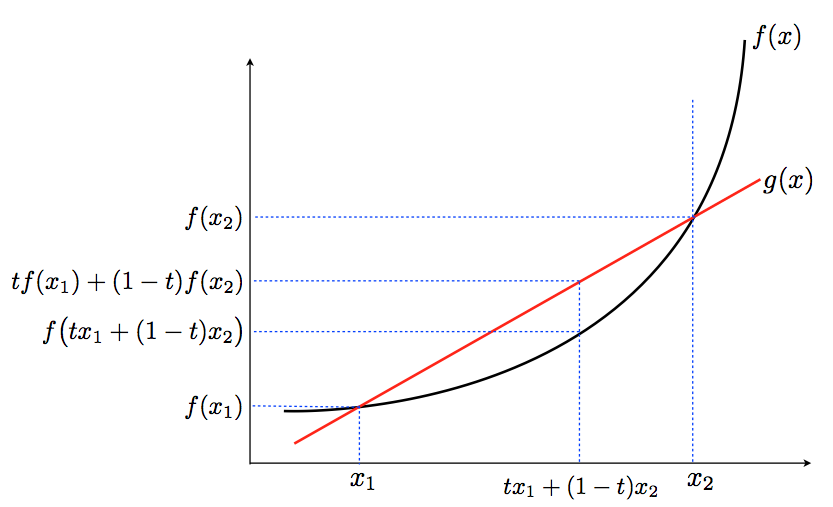
\includegraphics[width=.30\textwidth]{convex.png}
\end{figure}
	\item The \textbf{convex hull} of a set X of points in the Euclidean plane or Euclidean space is the smallest convex set that contains X.
	\item Polygon is a plane figure (2D) that is bounded by a finite chain of straight line segments (edges or sides) meeting at vertices and closing in a loop to form a closed chain or circuit.
	\item A \textbf{polytope} is a geometric object with flat sides which generalise the 2D polygon in n-dimensional.
	\item Convex Polytope is a polytope whose point form a convex set. It can be written in equation form as $Ax \leq b$ which correspond to a linear programming constraint.
\end{itemize}
\begin{figure}[H]
    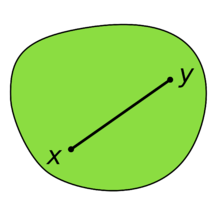
\includegraphics[width=.11\textwidth]{220px-Convex_polygon_illustration1.png}
    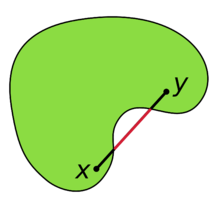
\includegraphics[width=.11\textwidth]{220px-Convex_polygon_illustration2.png}
    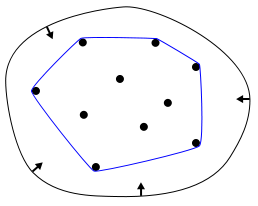
\includegraphics[width=.11\textwidth]{258px-ConvexHull_svg.png}
    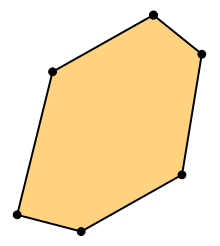
\includegraphics[width=.11\textwidth]{A_2-dimensional_polytope_svg.png}
    \caption{(a) convex set,(b) not convex set,(c) convex hull,(d) 2D-polytope}
\end{figure}


	\subsection{Fermat's theorem, Euler-Lagrange equation}
\begin{itemize}
	\item \textbf{Fermat's theorem} states that at any point where a differentiable function attains a local extremum, its derivative is zero. Let $f\colon (a,b) \rightarrow \mathbb{R}$ be a differentiable function on an extremum $x_0 \in (a,b)$, then $\displaystyle f'(x_0) = 0$
	
	\item \textbf{Euler-Lagrange equation} is a partial differential equation whose solutions are the functions for which a given functional is stationary. In 1D, 
$$ \frac{\partial F}{\partial f} - \frac{\mathrm{d}}{\mathrm{d}x} \frac{\partial F}{\partial f'} = 0 $$
	The idea behind the equation is that we want to find the function $f(x)$ which minimize (or maximize) a real-valued function $F \colon (x,f(x),f'(x))\mapsto \mathbb{R}$. In order to find it, we set the derivative of the integral of $F$ to zero, which end up in a partial derivative function known as the Euler-Lagrange equation.
\end{itemize}



	\subsection{Method of Lagrange multipliers}
Lagrange method is used for first order derivable continuous function with only equality constrains ($h(\mathbf{x})=0$).

\begin{figure}[H]
	\centering
    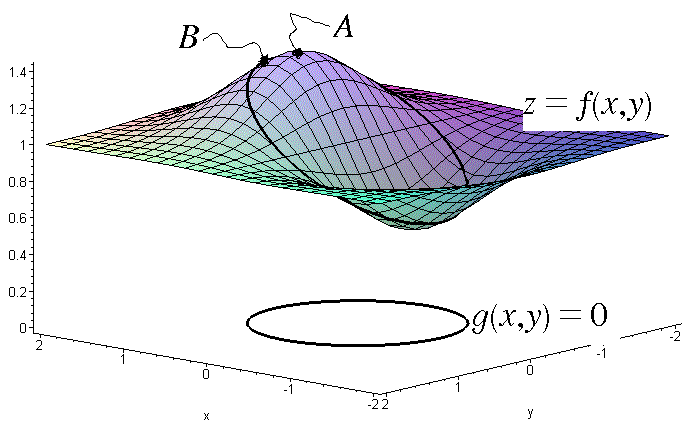
\includegraphics[width=.20\textwidth]{lagrange.png}
    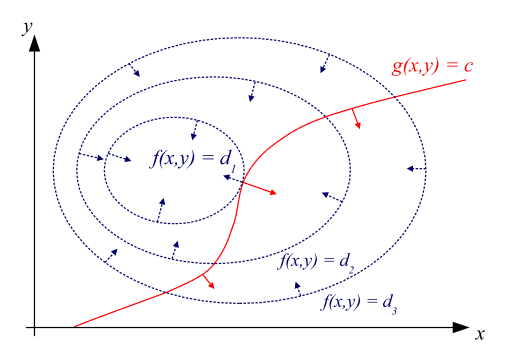
\includegraphics[width=.20\textwidth]{LagrangeMultipliers2D.png}
\end{figure}
 The idea is that at the solution ($\mathbf{x^*}$), the gradient vector of both function ($f,h$) will have the same direction: 
 $$\nabla f(\mathbf{x^*}) = -\mathbf{\lambda} \cdot \nabla h(\mathbf{x^*})$$
Where $\lambda$ is a multiplier called the Lagrange multiplier. In order to find this point, we can use the Lagrange function :
$$ \Lambda(\mathbf{x},\mathbf{\lambda}) = f(\mathbf{x}) + \mathbf{\lambda} \cdot h(\mathbf{x})$$

which will have a stationary point at the solution 
$$\nabla_{\mathbf{x},\lambda} \Lambda(\mathbf{x^*},\mathbf{\lambda^*})=0$$
Expending this equation rise to $n+1$ equations with $n+1$ variable to solved. Note that $\nabla_\lambda \Lambda=0$ force $h(\mathbf{x})=0$. Multiple constraint can be added and Karush-Kuhn-Tucker generalized it for inequality constraint





	\subsection{Karush-Kuhn-Tucker conditions}
The KKT approach generalizes the method of Lagrange multipliers to inequality constraints.
 $$\nabla f(\mathbf{x^*}) = - \sum_{j=1}^l \lambda_j \nabla h_j(\mathbf{x^*}) -\sum_{i=1}^m \mu_i \nabla g_i(\mathbf{x^*})$$

For the inequality constraint, we can show that $\mu_i g_i (\mathbf{x^*}) = 0$ because $\mu_i=0$ when the solution is outside the inequality space ($g_i(\mathbf{x^*}) < 0$, constraint null) and otherwise, $g_i (\mathbf{x^*}=0$ because the solution is at the boarder of the space.

Because the solution on $g_i(\mathbf{x})>0$ or $g_i(\mathbf{x})=0$, $\mu_i$ can only be zero or greater than zero ($\nabla g_i(\mathbf{x})$ has opposite sign to $\nabla f(\mathbf{x})$)
 
 \begin{figure}[H]
	\centering
    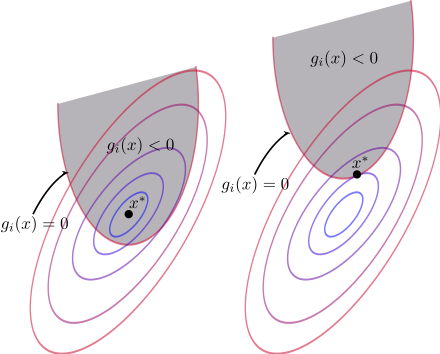
\includegraphics[width=.26\textwidth]{440px-Inequality_constraint_diagram.png}
    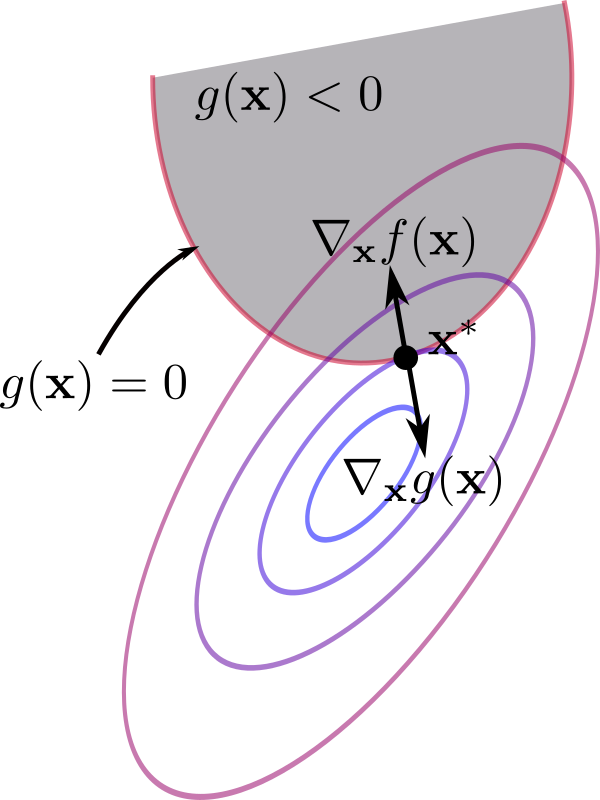
\includegraphics[width=.15\textwidth]{signofkkt.png}
\end{figure}

	\subsection{Lagrange duality}
Duality means that optimization problems may be viewed from either of two perspectives, the primal problem or the dual problem (the duality principle). The solution to the dual problem provides a lower bound to the solution of the primal (minimization) problem.

$$ \Lambda(\mathbf{x},\mathbf{\lambda},\mu) = f(\mathbf{x})  + \sum_{j=1}^l \lambda_j \nabla h_j(\mathbf{x}) +\sum_{i=1}^m \mu_i \nabla g_i(\mathbf{x})$$

$$\sum_{j=1}^l \lambda_j h_j(\mathbf{x^*}) +\sum_{i=1}^m \mu_i  g_i(\mathbf{x^*}) \le 0$$

and therefore the Lagrange dual function is the lowest bound of the primal problem:
$$g(\lambda,\mu) = \inf \Lambda(\mathbf{x},\lambda,\mu) \le \Lambda(\mathbf{x^*},\mathbf{\lambda},\mu) \le f(\mathbf{x^*})$$

	\subsection{Markov-chain Monte Carlo (MCMC)}
\begin{itemize}
	\item Monte Carlo are broad class of algorithm that rely on repeated random sampling to obtain numerical results.
	\item Markov-chain is a random process that undergoes transitions from one state to another where the probability distribution of the new state depends only on the current state and not on the sequence of events that preceded it (Markov property).
$$\Pr(x_{n+1}\mid x_1, \ldots, x_n) = \Pr(x_{n+1}\mid X_n)$$ 
	\item MCMC combine both properties.
\end{itemize}













\newpage
\section{Problem Categorisation}
	\subsection{Global vs Local}
Global (or absolute) method intend to find the best estimate over the whole space rather than part of the parameter space (local or relative). Strict extremum is the only one best value.(
$$f(\mathbf{x}^*) \underbrace{\leq}_{< \mbox{ for strict}} f(\mathbf{x^*+\epsilon}) \qquad  \left\{
  \begin{array}{lr}
    \exists \epsilon>0 & \mbox{local}\\
    \forall \epsilon>0 & \mbox{global}
  \end{array}
\right.
 $$





	\subsection{Linear (LP), non-linear (NLP) and quadratic programming}
LP is an convex optimization technique used with linear objective function, subject to linear equality and/or inequality constraints. 
 \begin{align*}
& \text{minimize}   && f(\mathbf{x})=\mathbf{c}^\mathrm{T} \mathbf{x}\\
& \text{subject to} && A \mathbf{x} \leq \mathbf{b} \\
& \text{and} && \mathbf{x} \ge \mathbf{0}
\end{align*} 
These constraint correspond to a convex polytope. Because of the OF is linear (can always decrease in a certain direction), we know that it minimum occur at a boundary of the constraint polytope.
\begin{figure}[H]
	\centering
    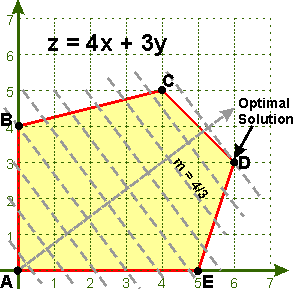
\includegraphics[width=.20\textwidth]{linear.png}
\end{figure}

For quadratic problem, the OF is describe with:
$$ f(\mathbf{x})=\mathbf{x}^T Q\mathbf{x} + \mathbf{c}^T \mathbf{x}$$
The constrain are usually the same as linear but could also be quadratic



	\subsection{Heuristic and Meta-heuristic}
Heuristic method search for an approximate solution ("good enough") by trading optimality (the best), completeness (all), accuracy, or precision for speed. In order to find this approximate, informations about the problem are required. Meta-heuristic are called approximation (rather than approximate) in the sense that they are proven close solution, which can therefore be applied to any problem without adaptation.


	\subsection{Pattern search}
Pattern search (also called Direc-Search) is a family of optimization that do not require the gradient of the problem. 

	\subsection{Stochastic vs Deterministic}
In stochastic optimization, unknown parameter are handle with uncertainty and pdf while 


	

	\subsection{Multi-objective optimization and Pareto Front}
For non-trivial multi-objective optimization problem, there does not exist a single solution that simultaneously optimizes each objective. A solution is called Pareto optimal (or efficient) if none of the objective functions can be improved without degrading some of the other objective values. Vector optimization is the generalized case.


	\subsection{Rate of Convergence} \label{subsec:rateofconvergence}
Suppose that the sequence ${x_k}$ converges to the number L. Classification:
$$\lim_{k\to \infty} \frac{|x_{k+1}-L|}{|x_k-L|} = \mu$$
\begin{itemize}
	\item \textbf{Linear}, $\mu \in (0, 1)$
	\item \textbf{Superlinearly}, $\mu=0$. We say that the sequence converges with order $q$ to L for $q>1$ if: ($q = 2$ is quadratic convergence)
	$$ \lim_{k\to \infty} \frac{|x_{k+1}-L|}{|x_k-L|^q} = \mu \quad  \text{with} \mu > 0$$
	\item \textbf{Sublinearly}, $\mu=1$. The sequence converges logarithmically to L if 
	$$ \lim_{k\to \infty} \frac{|x_{k+2} - x_{k+1}|}{|x_{k+1} - x_k|} = 1$$
\end{itemize}
\begin{figure}[H]
	\centering
    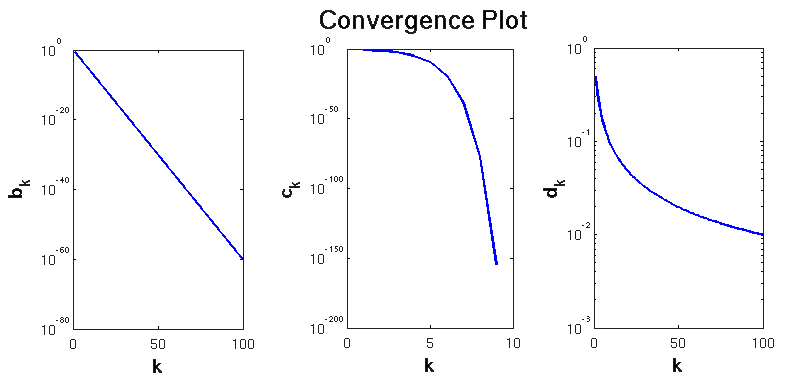
\includegraphics[width=.40\textwidth]{ConvergencePlots.png}
\end{figure}













\newpage
\chapter{ }

\section{Optimization algorithms}
	\subsection{Simplex Algorithm}
\emph{Linear programing, }\\
One of the top 10 algorithm of the twentieth century, Simplex algorithm solved linear programme (LP) using the property that the minimum is always at a vertex.
\begin{framed}\begin{algorithmic}
\State Start on a vertex of the polytope
\While{One of the neighbouring vertices has a lower OF}
	\State Move to the new vertex
\EndWhile
\end{algorithmic}\end{framed}
Numerical solution for this involve simplex tableaux and pivot operations. The revised simplex method implement the same mathematical expression but in matrices form. Other method which uses this basic idea is the path-following algorithms.



\section{Gradient-Based Algorithm (Iterative methods)}

	\subsection{Gradient descent}
\emph{Gradient-based, differentiable}\\
Gradient descent is an interative method which start with a point and move toward the negative gradient proportional to the step size ($\gamma_n$)
$$\mathbf{x}_{n+1}=\mathbf{x}_n-\gamma_n \nabla f(\mathbf{x}_n)$$
In some case, the optimal step size can be computed analytically.
\begin{figure}[H]
	\centering
    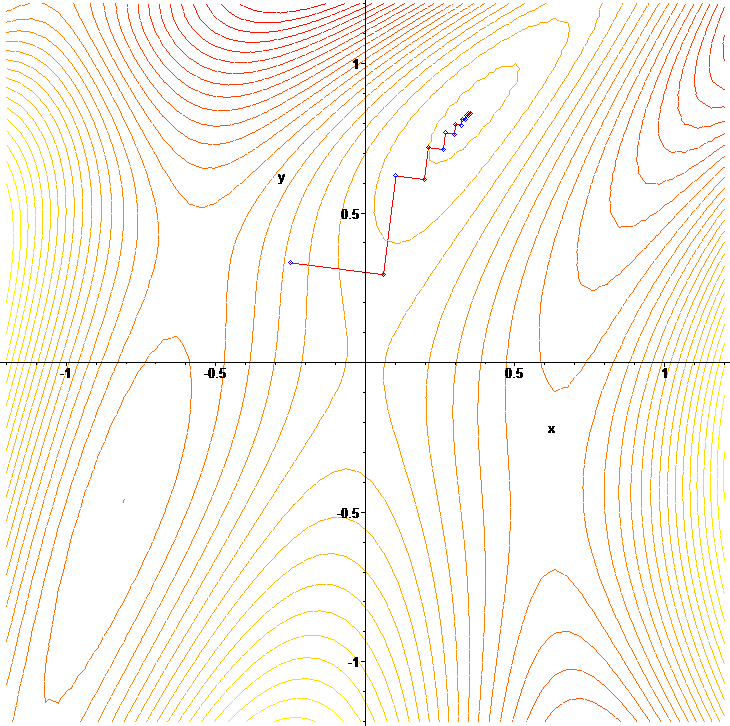
\includegraphics[width=.16\textwidth]{Gradient_ascent_(contour).png}
    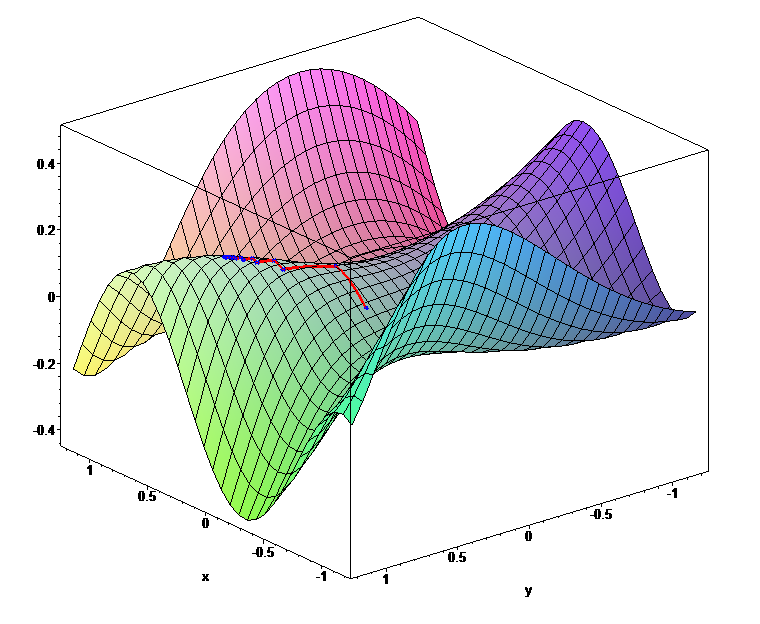
\includegraphics[width=.20\textwidth]{Gradient_ascent_(surface).png}
\end{figure}


	\subsection{Conjugate gradient method}
\emph{linear or quadratic, gradient-based, iterative, }\\
CGM is solving either an inverse problem for linear problem ($\mathbf{x|Ax=b}$) or an optimization problem for the quadratic expression whose gradient is the linear problem $\nabla f(\mathbf{x)=Ax-b}$. This is equivalent as the minimum of $f$ will be found when his gradient is null. 

$$ f(\mathbf{x}) = \frac12 \mathbf{x}^\mathrm{T} \mathbf{A}\mathbf{x} - \mathbf{x}^\mathrm{T} \mathbf{b} $$ 
The matrix $\mathbf{A}$ need to be symmetric (i.e., $\mathbf{A}^T = \mathbf{A}$), positive definite (i.e. $\mathbf{x}^T\mathbf{A}\mathbf{x} > 0 \quad \forall \mathbf{x}\not=0 \in \mathbb{R}^n$), and real (i.e. $\mathbf{A} \in \mathbb{R}^n$).


In the gradient descent, the iterative approach would use a direction of search $\mathbf{p}_n=\nabla f(\mathbf{x})=-(\mathbf{Ax}_n-\mathbf{b})$
We can see that this expression is the residual of the linear problem denoted $ \mathbf{r}_{n}=\mathbf{b}-\mathbf{Ax}_n$
$$\mathbf{x}_{n+1}=\mathbf{x}_n+\gamma_n(\mathbf{b}-\mathbf{Ax}_n)$$
But in CGM, the new direction of search need to be a conjugate gradient of the previous one $\langle \mathbf{p}_n,\mathbf{p}_k\rangle_{A}=0, \quad \forall k<n $. This new direction can be found by subtraction the projection of the gradient to the previous direction:
$$ \mathbf{p}_{n} = \mathbf{r}_{n} - \sum_{i < n} \mathrm{proj}_{\mathbf{p}_i}\,(\mathbf{r}_n) =\mathbf{r}_{n} - \sum_{i < n}\frac{\mathbf{p}_i^\mathrm{T} \mathbf{A} \mathbf{r}_{n}}{\mathbf{p}_i^\mathrm{T}\mathbf{A} \mathbf{p}_i} \mathbf{p}_i $$

And finally, this gave us:
 $$\mathbf{x}_{n+1} = \mathbf{x}_n + \alpha_n \mathbf{p}_n, \qquad 
 \alpha_{n} = \frac{\mathbf{p}_n^\mathrm{T} \mathbf{b}}{\mathbf{p}_n^\mathrm{T} \mathbf{A} \mathbf{p}_n}$$


The advantage of Conjugate gradient method over Newton's method is that matrix is not store and therefore Conjugate Gradient Method is used when factorization is not feasible.



The biconjugate gradient method provides a generalization to non-symmetric matrices. 
Various nonlinear conjugate gradient methods seek minima of nonlinear equations.


 
 
	\subsection{Newton's Method}
Newton's Method is a method for finding successively better approximations to the roots (or zeroes) of a real-valued differentiable function.
$$\mathbf{x}_{n+1} = \mathbf{x}_n - \frac{f(\mathbf{x}_n)}{f'(\mathbf{x}_n)} $$

		\subsubsection{Analysis}
Newton's Method come from  \textbf{Taylor Second order expension}
$$f(\mathbf{x}) = f(\mathbf{x}_n) + f^\prime(\mathbf{x}_n)(\mathbf{x} - \mathbf{x}_n) + R_1  $$
where the remainder is 
$$R_1 = \frac{1}{2!}f^{\prime\prime}(\mathbf{\xi}_n)(\mathbf{x} - \mathbf{x}_n)^{2} \quad \text{with } \xi\in \mathbb{R}, |\mathbf{x} - \xi_n| < |\mathbf{x}-\mathbf{x}_n|$$
By setting $\epsilon_n=\mathbf{x-x}_n$, and $f(\mathbf{x})=0$. we can find that under some condition the rate of convergence is quadratic\textsuperscript{\ref{subsec:rateofconvergence}}
$$\frac{|\epsilon_{n+1}|}{\epsilon_n^2}=\frac{|f''(\xi_n)|}{2|f'(\mathbf{x}_n)|}$$


		\subsubsection{Failure}
Failure to converge can be caused by a stationary point ($f'(\mathbf{x})=0$), a poor initial estimate, overshooting or  cyclic iteration.

If the derivative is unknown, the \textbf{secant method},  is a simplistic solution which replace the derivative with a backward finite difference approximation :
$$ \mathbf{x}_n=\mathbf{x}_{n-1}-f(\mathbf{x}_{n-1})\frac{\mathbf{x}_{n-1}-\mathbf{x}_{n-2}}{f(\mathbf{x}_{n-1})-f(\mathbf{x}_{n-2})}$$

To avoid overshooting, a small step $ \gamma_n \in (0,1)$ (which can change at each iteration) can be add:
$$\mathbf{x}_{n+1} = \mathbf{x}_n - \gamma_n \frac{f(\mathbf{x}_n)}{f'(\mathbf{x}_n)}$$

		\subsubsection{Generalization}
For a system of k non-linear equations $\mathbf{f}$ of k variable $\mathbf{x}$, the derivative $\mathbf{f}'$ is called the Jacobian matrix $\mathbf J_{i,j} = \frac{\partial f_i}{\partial x_j}$ and Newton's method become:
$$\mathbf J_f (\mathbf{x}_{n+1} - \mathbf{x}_n) = -\mathbf{f}(\mathbf{x}_n)$$

For under-determined problem (number of equation smaller than number of variable), the generalized inverse \ref{} of the non-square Jacobian matrix $\mathbf{J^+ = (( J J^\mathrm{T} J)}^{-1}) \mathbf{J^\mathrm{T}}$ instead of the inverse of $\mathbf J$.

	\subsection{Gauss-Newton Method}
In over-determined problem, the Gauss-Newton method simplify the Newton method to minimize a function in a least square sense (instead of finding the root). 
In least-squre problem, the function to minimized is sum of square of the residual $\mathbf{r}(\mathbf{x})$ with $m$ parameters $\mathbf{x}$
$$f\colon \mathbb{R}^m \rightarrow \mathbb{R} \qquad f(\mathbf{x})=\sum_i \mathbf{r}_i^2(\mathbf{x})$$
$$\mathbf{J}_f\colon \mathbb{R}^m \rightarrow \mathbb{R}^m \qquad \mathbf{J}_f(\mathbf{x})=2\sum_i r_i(\mathbf{x}) \frac{\partial \mathbf{r}_i(\mathbf{x})}{\partial \mathbf{x}}$$
$$\mathbf{H}_f\colon \mathbb{R}^m \rightarrow \mathbb{R}^{m\times m} \qquad \mathbf{H}_f(\mathbf{x})=2\sum_{i} \left(\frac{\partial r_i}{\partial \beta_j}\frac{\partial r_i}{\partial \beta_k}+r_i\frac{\partial^2 r_i}{\partial \beta_j \partial \beta_k} \right).$$
[...]

Starting from an optimization version of Newton method, where the function to minimized is the sum of square of the residual $f(\mathbf{x})=\sum r_i^2$, where the residual is de difference between $x$ and known data $d$, $r_i=x_i-d_i$
$$\mathbf{x}_{n+1} = \mathbf{x}_n - \frac{f'(\mathbf{x}_n)}{f''(\mathbf{x}_n)} $$
where $f' = 2 \sum r_i \frac{\partial r_i}{\partial \mathbf{x}}$ and $f'' = 2 \sum r_i \frac{\partial r_i}{\partial \mathbf{x}}$
It can be shown that the Hessian can be approximate by $2\mathbf{J}_f^\mathrm{T}\mathbf{J}_f$
$$ \mathbf{x}_{n+1} = \mathbf{x}_n  +  (\mathbf{J}_f^\mathrm{T}\mathbf{J}_f)^{-1}\mathbf{J}_f^\mathrm{T} f(\mathbf{x}_n)$$


We can observe ... The Jacobian became an orthogonal matrix which imply $\mathbf{J}_f^\mathrm{T}=\mathbf{J}_f^{-1}$ and $(\mathbf{J}_f^\mathrm{T}\mathbf{J}_f) =\mathbf I$. The Gaussian-netwon simplyfyied in the generalized solution of Newton.

This relationship can be found when looking at minima (stationary point, $f'=0$).The Newton method is reformulate with the Hessian $\bold H_{i,j} = \frac{\partial^2 f}{\partial \mathbf x_i \partial \mathbf x_j}$ replacing $f$ by this jacobienne:


	\subsection{Levenberg–Marquardt algorithm}
The LMA interpolates between the Gauss–Newton algorithm (GNA) and the method of gradient descent by using a dumping factor $\lambda$ (Levenberg):
$$ \mathbf{x}_{n+1} = \mathbf{x}_n  +  (\mathbf{J}_f^\mathrm{T}\mathbf{J}_f + \lambda_n \mathbf{I})^{-1}\mathbf{J}_f^\mathrm{T} f(\mathbf{x}_n)$$
The (non-negative) damping factor, λ, is adjusted at each iteration. If reduction of S is rapid, a smaller value can be used, bringing the algorithm closer to the Gauss–Newton algorithm, whereas if an iteration gives insufficient reduction in the residual, λ can be increased, giving a step closer to the gradient descent direction.
Marquardt improve this by weighting each dumping factor depending on the gradient (convergence) in each direction
$$ \mathbf{x}_{n+1} = \mathbf{x}_n  +  (\mathbf{J}_f^\mathrm{T}\mathbf{J}_f + \lambda_n \mathrm{diag}(\mathbf{J}_f^\mathrm{T}\mathbf{J}_f) )^{-1}\mathbf{J}_f^\mathrm{T}$$

The LMA is more robust than the GNA, which means that in many cases it finds a solution even if it starts very far off the final minimum. For well-behaved functions and reasonable starting parameters, the LMA tends to be a bit slower than the GNA. LMA can also be viewed as Gauss–Newton using a trust region approach.

	\subsection{Quasi-Newton Method} 
Strictly, any method that replaces the exact Jacobian with an approximation can is a quasi-newton method. But in practice, Variable Metric Methode is accumulating information to build up a better approximation of the inverse Hessian 

\section{Heuristics}


	\subsection{Particle swarm-essaims de particule}
\emph{meta-heuristique, not gradient based, no guarantee of global, Swarm intelligence, evolutionary computing}\\
A set of S particles (candidate solutions) are moved around the search-space $[x_{min}, x_{max}]$ with its velocity ($v_i^s$) which is computed according to its current position ($x_i^s$), its best estimate ($x_b^s$) as well as the global best estimate ($x_b^b$).

\begin{framed}\begin{algorithmic}
\For{ each particle $s=0,\ldots,S$} 
	\State $x_0^s \gets \mathcal{U}(x_{min}, x_{max})$ \Comment{position}
	\State $x_{b}^s \gets x_0^s$ \Comment{best position}
	\State $v_0^s \gets \mathcal{U}(-|x_{min}, x_{max}|, |x_{min}, x_{max}|)$ \Comment{velocity}
	\If {$f(x_0^s) < f(x_b^b)$}
    	\State $x_b^b \gets x_0^s $
    \EndIf
\EndFor

\While{$criterion(i, f(x_b), f(x_{b,new})/f(x_{b,old}))$}
\State $i \gets i+1$
\For{ each particle $s=0,\ldots,S$}
	\State $r_b, r_{bb} \gets \mathcal{U}(0,1)$
	\State $v_i^s \gets \omega v_{i-1}^s + \phi_b r_b (x_b^s - x_{i-1}^s) + \phi_{bb} r_{bb} (x_b^b - x_{i-1}^s)$ \Comment{update velocity}
	\State $x_i^s \gets x_{i-1}^s + v_i^s$ \Comment{update position}
	\If {$f(x_i^s)< f(x_{b}^s)$}
    	\State $x_{b}^s \gets x_i^s$
    	\If {$f(x_i^s)< f(x_{b}^b)$}
    		\State $x_{b}^b \gets x_i^s$
    	\EndIf
    \EndIf
\EndFor
\EndWhile
\end{algorithmic}\end{framed}

Method exist to compute best parameters($r_{b},r_{bb},\omega, \phi_b, \phi_{bb}$).
	\subsection{Evolutionist algorithm}
\emph{Population-based, stochastic, meta-heuristic}\\
An evolutionist algorithm uses mechanisms inspired by biological evolution, such as reproduction, mutation, inheritance, crossover, and selection.
\begin{framed}\begin{algorithmic}
\State Generate randomly first generation 
\While{criteria not met (time,fitness...)}
	\State - Evaluate the fitness of each individual
	\State - Select the best-fit individuals for reproduction
	\State - Breed new individuals through crossover and mutation operations to give birth to offspring
	\State - Replace least-fit population with new individuals
\EndWhile
\end{algorithmic}\end{framed}
Genetic algorithm and evolutionist strategie are different in the sence that recominbaison is randomized in genetic while evlutionist uses co-evolution in order to find convergence.


Read more : Schulze-Riegert and Ghedan, 2007










	\subsection{Golden Section Search}
	\emph{Unimodal function, }\\
This method used for unimodal function successively narrows the range of values containing the solution by sampling function values for triples of points whose distances form a golden ratio. (see also Fibonacci search).
\begin{figure}[H]
	\centering
    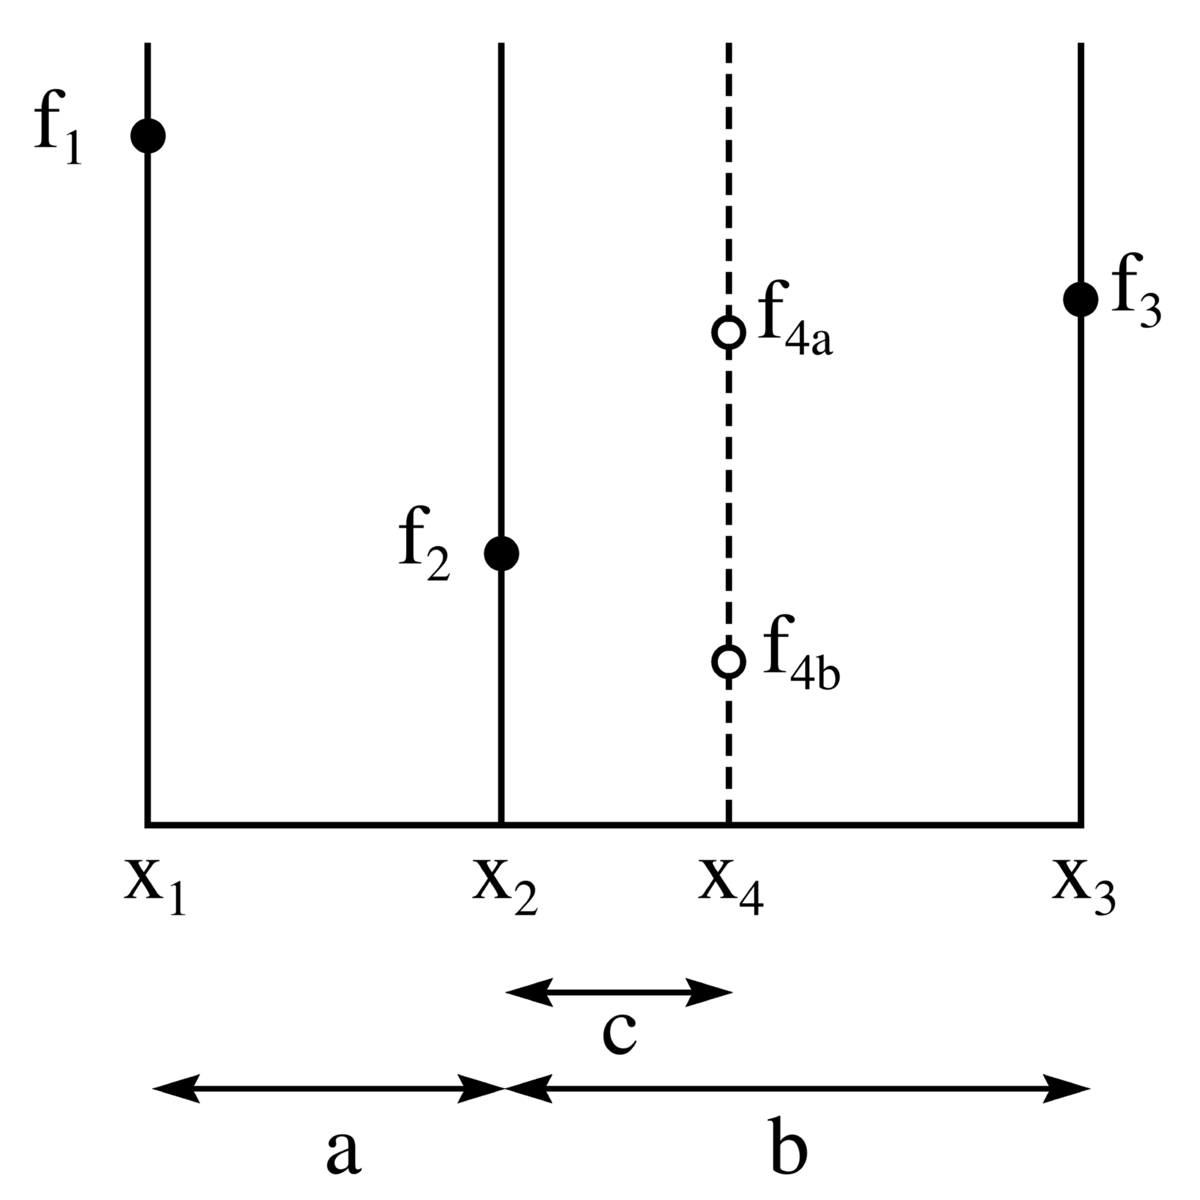
\includegraphics[width=.40\textwidth]{GoldenSectionSearch.png}
\end{figure}

If the interval is divided by two (instead of forming a golden ratio), the method is called \textbf{Bisection method}.



	\subsection{Simulated annealing-recuit simulé}
\emph{meta-heuristic, global, stochastic}\\
\begin{framed}\begin{algorithmic}
\State $x_{b} \gets x_0$
\While{$criterion(i, f(x_b), f(x_{b,new})/f(x_{b,old}))$}
	\State $x_i \gets neighbour(x)$
	\If {$\Pr(f(x), f(x_i),i) > \mathcal{U}(0, 1) $}
    	\State $x_{b}\gets x_i$
    \EndIf
\EndWhile
\end{algorithmic}\end{framed}
where:
\begin{itemize}
	\item $x_{b}$ is the current best estimate and $x_i$ is the proposed new estimate
	\item $criterion()$ return true if none criteria is met otherwise false and stop the algorithm
	\item $neighbour()$ is a function returning a new proposed estimate from the current estimate. This is a sort of perturbation function.
	\item $\Pr(f(x), f(x_i),i)$ is the acceptance probabilities. 
	\begin{itemize}
		\item The probability increase with a increase in the difference of the OF of the new estimate :$(f(x)-f(x_i)) \nearrow, \Pr \nearrow$. ie: best estimate, best chance to be accepted
		\item Usually, if $f(x)>f(x_i)$, $\Pr=1$, ie: better estimate, sure to be accepted.
		\item At the beginning, acceptance for worse estimate allow to explore more globally but along the iteration, it become more and more difficult to converge.
	\end{itemize}
\end{itemize}
Method to find good neighbour and acceptance exist.



 
 
 
 



\bibliographystyle{apalike}
\bibliography{citations}	
	

\end{document}
